\chapter{Graph Construction}
\label{ch:graph_construction}

\section{Overview}
\label{sec:graph_overview}

The graph construction phase is the third and final stage of the
analysis pipeline. It receives as input the module hierarchy
$\vec{\mathcal{M}} \in \mathcal{D}$ produced by the extraction phase and
refined by the name resolution phase, in which all type references
$\tau$ have been resolved to their final states (\texttt{Resolved},
\texttt{External}, \texttt{Primitive}, or \texttt{Failed}). The output is
a \textbf{Dependency Graph} $\mathcal{G} = (V, E)$, a directed multigraph
where vertices $V \subset \mathcal{C}$ represent software components and
edges $E$ represent semantic dependencies between components.

Formally, the graph construction function $\gamma$ is defined as:
$$\gamma : \vec{\mathcal{M}} \to \mathcal{G}$$

The construction pipeline operates in two sequential traversal passes
followed by a post-processing phase:
\begin{enumerate}
  \item \textbf{Pass 1 (Node Extraction)}: The module tree is
    recursively traversed to collect all workspace components (modules,
    structured types, functions, fields, and type aliases) into the vertex
    set $V$, computing their globally unique qualified names.
  \item \textbf{Pass 2 (Edge Generation)}: The tree is traversed a second
    time to inspect resolved references within signatures and code blocks,
    emitting directed dependency edges of the form
    $e = \langle \pi_{src}, \pi_{tgt}, k \rangle \in E$.
  \item \textbf{Post-processing}: Ensures referential integrity by
    dynamically adding implicit endpoints (\texttt{Primitive} and
      \texttt{External} types referenced by edges but absent from the
    workspace) to $V$, and deduplicates identical edges.
\end{enumerate}

The overall architecture of this construction pipeline is summarized
in Figure~\ref{fig:graph_construction_pipeline}.

\begin{figure}[htpb]
  \centering
  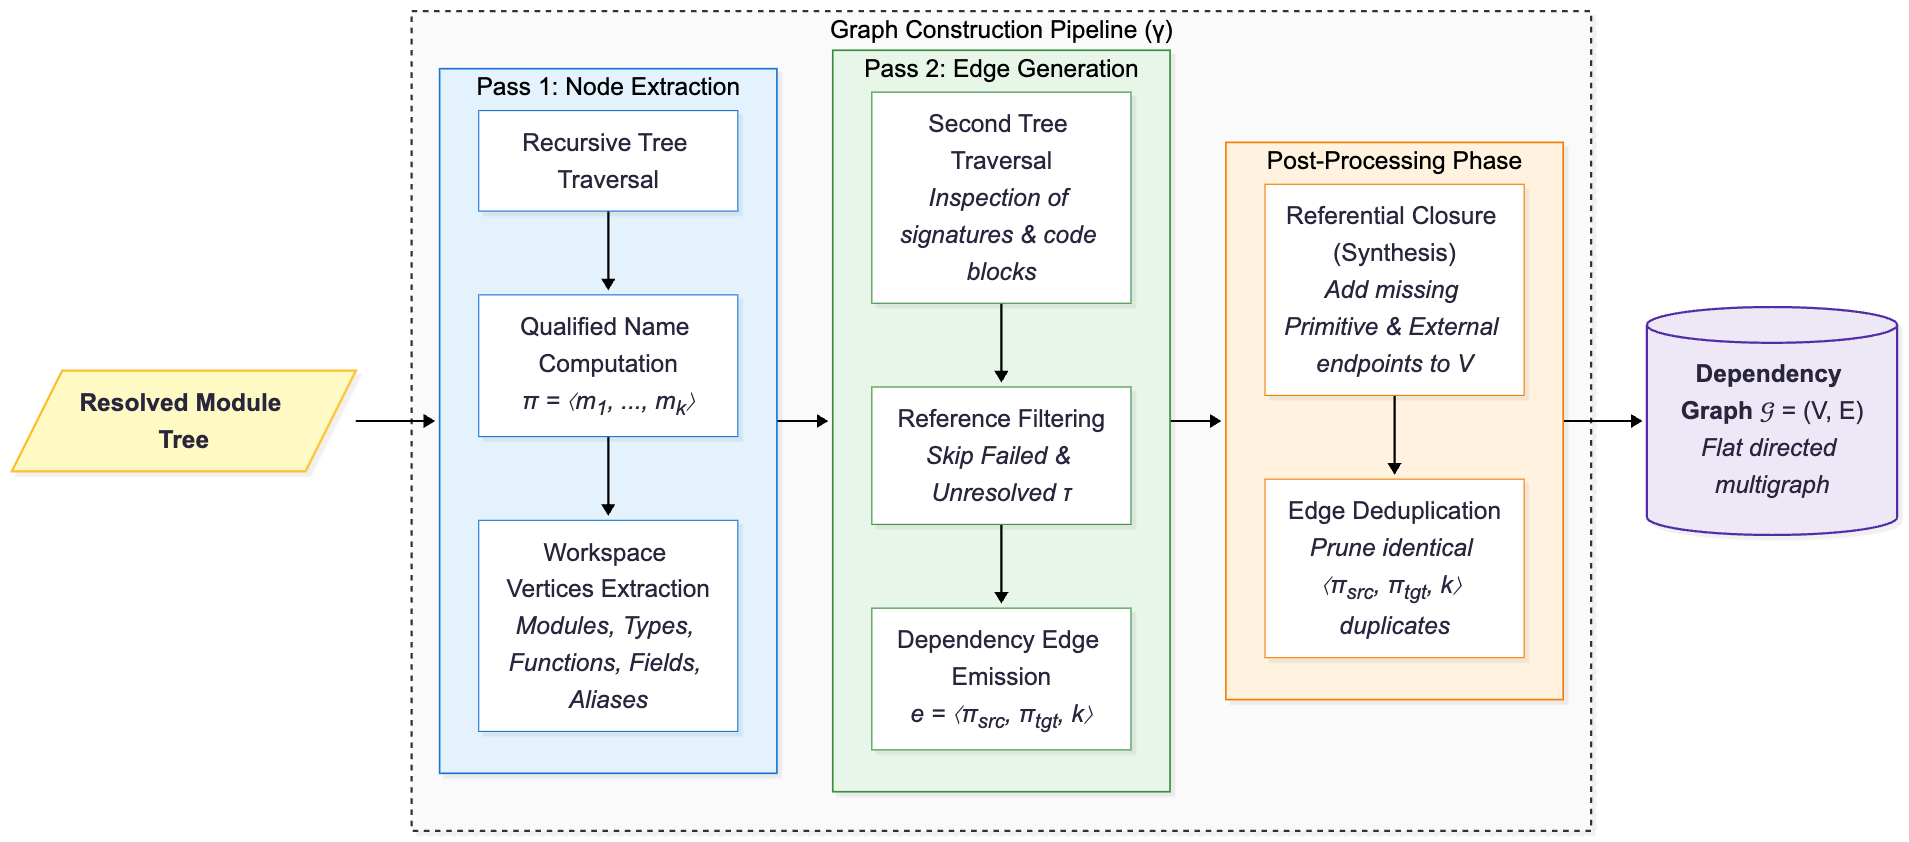
\includegraphics[width=\textwidth]{images/graph_construction/graph_construction_pipeline.png}
  \caption{High-level pipeline of the graph construction phase
    ($\gamma$). The resolved module hierarchy ($\vec{\mathcal{M}} \in
    \mathcal{D}$) undergoes a first traversal pass to extract workspace
    vertices ($V$), a second pass to emit directed dependency edges
    ($E$), and a post-processing stage that guarantees referential
  closure and eliminates duplicate edges.}
  \label{fig:graph_construction_pipeline}
\end{figure}

\section{Node Flattening}
\label{sec:node_flattening}

The Intermediate Representation is structured as a recursive tree of
modules ($\mathcal{M}$), where each module can contain sub-modules,
structured types, functions, type aliases, and free variables. The
dependency graph, however, requires a flat set of vertices. The
flattening algorithm recursively traverses the module tree and
promotes every component to an independent graph node.

\subsection{Qualified Name Computation}

During flattening, each component's name is recomputed as a globally
unique \textbf{Qualified Name} $\pi$ by prepending the names of all
ancestor modules. For instance, a class \texttt{User} declared inside
module \texttt{auth}, which is itself nested in the root module,
receives the qualified name $\langle \texttt{auth}, \texttt{User}
\rangle$. The root module name is filtered out from the prefix to
avoid redundant path segments.

This globally qualified naming scheme guarantees that every vertex in
the graph has a unique identifier, even when multiple entities share
the same local name across different modules.

\subsection{Entities Promoted to Vertices}

The flattening process generates vertices for the following five IR
constructs extracted from the workspace:
\begin{itemize}
  \item \textbf{Modules} ($\mathcal{M}$): Every module and sub-module
    in the hierarchy becomes a vertex of type \texttt{Module}.
  \item \textbf{Structured Types} ($\mathcal{S}$): Every class,
    struct, interface, trait, enum, and enum variant becomes a vertex
    of type \texttt{StructuredType}. Nested types (inner classes,
    nested structs) are recursively flattened and promoted to
    independent vertices.
  \item \textbf{Functions} ($\mathcal{F}$): Every free function and
    every method declared inside a structured type becomes a vertex
    of type \texttt{Function}.
  \item \textbf{Fields} ($f$): Every field of a structured type and
    every free variable declared at module level becomes a vertex of
    type \texttt{Field}, carrying its qualified name and its type reference.
  \item \textbf{Type Aliases} ($\mathcal{A}$): Every type alias
    becomes a vertex of type \texttt{TypeAlias}.
\end{itemize}

Unlike the five entities above, \textbf{Implementation Blocks} ($\mathcal{X}$)
do not produce independent vertices in the graph. Instead, they act as
re-scoping containers: all methods, nested types, and type aliases declared
inside an \texttt{ImplBlock} are re-scoped under the target type's qualified
name and flattened into $V$ as if they were directly declared inside the target
structured type. Coupled with the dynamically synthesized vertices
described below,
the resulting vertex set $V$ covers all seven variants of the
universal component
domain $\mathcal{C}$.

\subsection{Dynamic Node Synthesis}

After the initial flattening, edges may reference types that are not
present as vertices in the workspace. This occurs when a component
depends on a primitive type (e.g., \texttt{int}, \texttt{bool},
\texttt{String}) or on an external type from a third-party library
(e.g., \texttt{java.util.List}, \texttt{std::collections::HashMap}).

To maintain referential integrity, the post-processing algorithm scans all
generated edges and identifies target endpoints that do not match any
existing workspace vertex:
\begin{itemize}
  \item If the target is recognized as a primitive type by the
    \textit{Primitive Registry} (introduced in Chapter
    \ref{ch:ir_formalization}), a \texttt{Primitive} node is synthesized.
  \item If the target corresponds to a certified third-party reference
    promoted through an explicit import directive, an \texttt{External}
    node is synthesized, representing an external dependency outside the
    analyzed workspace.
  \item Unresolvable references lacking a valid import directive remain in
    the \texttt{Failed} state and are pruned during edge generation, avoiding
    the creation of spurious or phantom nodes.
\end{itemize}

This approach guarantees that every emitted edge in the final multigraph
connects two valid endpoints in $V$, and that external dependencies are
explicitly observable as nodes.

\section{Edge Generation}
\label{sec:edge_generation}

The second sub-phase traverses the module tree recursively, inspecting every
component and its resolved type references to generate directed dependency
edges. Formally, the resulting dependency graph is a directed multigraph
$\mathcal{G} = (V, E)$, where $V \subset \mathcal{C}$ denotes the finite set of
flattened components and $E$ is the multiset of typed dependency edges.
Each edge $e \in E$ is formalized as a triple:
$$e = \langle \pi_{src}, \pi_{tgt}, k \rangle$$
where $\pi_{src}, \pi_{tgt} \in \Pi$ designate the qualified names of the
source and target components, and $k \in \text{Kind}$ identifies the semantic
nature of the dependency from the alphabet of fifteen supported
dependency kinds.

\subsection{Type Reference Filtering and Referential Integrity}

A fundamental invariant governs edge generation: dependency edges are
produced predominantly from type references in the terminal states
\texttt{Resolved}
and \texttt{External}.

During the Name Resolution phase (Chapter \ref{ch:name_resolution}),
a type reference is promoted to the \texttt{External} state if and
only if two conditions are strictly satisfied:
\begin{enumerate}
  \item The symbol's identifier matches an explicit import directive
    ($\delta \in \vec{\delta}_{imp}$) encountered during lexical
    scope climbing or module-level transitive import traversal;
  \item The imported path is verified to be absent from the
    workspace-wide Scope Tree ($\mathcal{E}$).
\end{enumerate}
This rigorous verification certifies that the entity genuinely
originates from an external third-party library or runtime platform
(e.g., \texttt{java.util.List}, \texttt{serde::Serialize}), rather
than an unresolvable local symbol or an extraction defect. For every
such certified reference, the edge generation phase emits a
dependency edge and post-processing dynamically synthesizes a
corresponding \texttt{External} vertex in $V$, making third-party
architectural couplings fully observable.

Conversely, references in the \texttt{Failed} state (symbols that
  could neither be located in the workspace hierarchy nor substantiated
by any matching import directive), as well as un-evaluated
\texttt{Unresolved} references with empty path specifications, are
deliberately skipped. This filtering ensures that unresolvable syntax
fragments or dynamic idioms do not introduce phantom nodes or
spurious dependencies into the architectural graph.

Finally, references categorized as \texttt{Primitive} by the
Primitive Registry ($\mathcal{P}$) generate dependency edges and
synthesize \texttt{Primitive} vertices in the multigraph, thereby
guaranteeing formal referential closure (every edge has valid source
and target endpoints in $V$). However, to prioritize high-level
software couplings and prevent visual clutter, primitive nodes and
their incoming edges are toggled off by default in the interactive visualizer.

For composite type references such as \texttt{Union($\vec{\tau}$)}
and \texttt{EvaluatedAccess($\tau_{path}, \tau_{type}$)}, the
algorithm recursively unpacks all inner references and generates
edges for each resolved target independently.

\subsection{Taxonomy of Dependency Edge Kinds}

The system defines 15 distinct edge kinds, organized into five
categories. Table \ref{tab:edge_taxonomy} provides a complete classification.

\begin{table}[htpb]
  \centering
  \small
  \begin{tabular}{|l|l|l|l|}
    \hline
    \textbf{Category} & \textbf{Edge Kind} & \textbf{Source} &
    \textbf{Target} \\ \hline
    \multirow{2}{*}{\textit{Structural}} & \texttt{ModuleContainment}
    & Module & Direct child \\ \cline{2-4}
    & \texttt{NestedIn} & StructuredType & Field, method, or nested
    type \\ \hline

    \multirow{2}{*}{\textit{Inheritance}} & \texttt{IsA} &
    StructuredType & Super type \\ \cline{2-4}
    & \texttt{Implements} & Module / StructuredType & Type / Trait \\ \hline

    \multirow{5}{*}{\textit{Type-Level}} & \texttt{UsesFieldType} &
    Field & Type of a field \\ \cline{2-4}
    & \texttt{UsesLocalType} & Function & Type of a local variable
    \\ \cline{2-4}
    & \texttt{UsesParamType} & Function & Type of a parameter \\ \cline{2-4}
    & \texttt{UsesReturnType} & Function & Return type \\ \cline{2-4}
    & \texttt{Aliases} & TypeAlias & Aliased target type \\ \hline

    \multirow{3}{*}{\textit{Behavioral}} & \texttt{Calls} & Function
    & Invoked function/type \\ \cline{2-4}
    & \texttt{Instantiates} & Function & Instantiated type \\ \cline{2-4}
    & \texttt{AccessesField} & Function & Accessed component \\ \hline

    \multirow{3}{*}{\textit{Auxiliary}} & \texttt{Imports} & Module /
    Type & Imported path \\ \cline{2-4}
    & \texttt{CastsTo} & Function & Cast target type \\ \cline{2-4}
    & \texttt{AnnotatedWith} & Any component & Annotation type \\ \hline
  \end{tabular}
  \caption{Complete taxonomy of the 15 dependency edge kinds,
  organized by category.}
  \label{tab:edge_taxonomy}
\end{table}

\subsubsection{Structural Edges}
Structural edges encode the hierarchical containment relationships of
the original source code:
\begin{itemize}
  \item \textbf{ModuleContainment}: Generated from a module to each
    of its direct children (sub-modules, structured types, free
    functions, free variables, and type aliases). The traversal is
    recursive: when a sub-module is encountered, the current module's
    qualified name is passed as the parent identifier.
  \item \textbf{NestedIn}: Generated from a structured type to each
    of its member fields, methods, and nested types. This edge captures
    structural ownership, establishing that a field or method ``belongs to''
    a class, or that an inner type is defined within the scope of an outer type.
\end{itemize}

\subsubsection{Inheritance Edges}
These edges model sub-typing, contract conformance, and decoupled
implementation extensions:
\begin{itemize}
  \item \textbf{IsA}: Generated from a structured type to each of its
    resolved super-types ($\vec{\tau}_{sup}$). In nominal object-oriented
    languages, this edge unifies class inheritance (\texttt{extends}),
    interface implementation (such as Java's \texttt{implements}), and
    trait super-traits into a single subtyping relation.
  \item \textbf{Implements}: Reserved for decoupled implementation blocks
    (\texttt{ImplBlock}), such as Rust's \texttt{impl} blocks or out-of-line
    type extensions. Because implementation blocks are dissolved during node
    flattening, two distinct edges model their semantic bindings:
    \begin{enumerate}
      \item An edge from the enclosing module to the target type
        ($M \xrightarrow{\text{Implements}} T$), capturing the architectural
        dependency that module $M$ provides an extension or method
        implementation
        for type $T$.
      \item If the block implements a trait or interface ($T \text{
        implements } \tau_{trait}$),
        an edge from the target type to the implemented trait
        ($T \xrightarrow{\text{Implements}} \text{Trait}$), recording
        contract fulfillment.
    \end{enumerate}
\end{itemize}

\subsubsection{Type-Level Edges}
Type-level edges capture static dependencies introduced through type
declarations:
\begin{itemize}
  \item \textbf{UsesFieldType}: Generated from a field $f$ (or a module-level
    free variable) to its resolved type. Under the fine-grained component
    model, the enclosing structured type is connected to its member field via
    a \texttt{NestedIn} edge, while the field itself carries the type
    dependency:
    for instance, if class \texttt{Car} has a field \texttt{engine: Engine},
    the graph contains \texttt{Car} $\xrightarrow{\text{NestedIn}}$
    \texttt{Car::engine}
    and \texttt{Car::engine} $\xrightarrow{\text{UsesFieldType}}$
    \texttt{Engine}.
  \item \textbf{UsesLocalType}: Generated from a function to the
    resolved type of each local variable declared in its body blocks.
    This edge kind was introduced to distinguish local variable
    dependencies from field-level dependencies.
  \item \textbf{UsesParamType}: Generated from a function to the
    resolved type of each of its formal parameters.
  \item \textbf{UsesReturnType}: Generated from a function to its
    resolved return type.
  \item \textbf{Aliases}: Generated from a type alias to its resolved
    target type, capturing the semantic binding between the alias and
    its original type.
\end{itemize}

Listing~\ref{lst:fine_grained_code} and
Figure~\ref{fig:dual_dependency_example} illustrate this distinction.
In Listing~\ref{lst:fine_grained_code}, the struct \texttt{Car}
declares a field \texttt{engine} of type \texttt{Engine} and a method
\texttt{drive} that invokes \texttt{self.engine.start()}. In the
resulting fine-grained dependency graph
(Figure~\ref{fig:dual_dependency_example}), \texttt{Car} contains its
members via \texttt{NestedIn} edges, while the type dependency
\texttt{UsesFieldType} originates strictly from the field node
\texttt{Car::engine} toward \texttt{Engine}. Concurrently, the method
\texttt{Car::drive} exhibits an \texttt{AccessesField} dependency
toward \texttt{Car::engine} and a \texttt{Calls} dependency toward
\texttt{Engine::start}.

\begin{lstlisting}[language=Rust, caption={Example illustrating fine-grained field and call dependencies.}, label={lst:fine_grained_code}]
struct Car {
    engine: Engine,
}

impl Car {
    fn drive(&self) {
        self.engine.start();
    }
}
\end{lstlisting}

\begin{figure}[htpb]
  \centering
  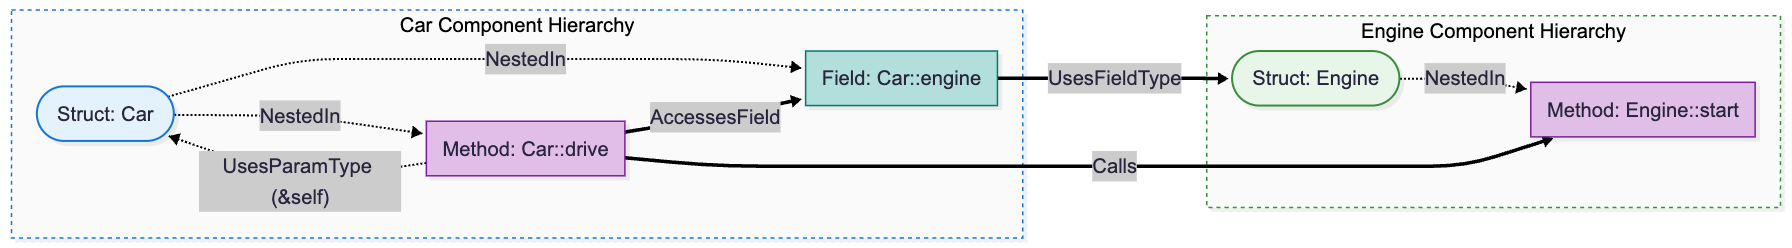
\includegraphics[width=\textwidth]{images/graph_construction/dual_dependency_example.png}
  \caption{Fine-grained dependency multigraph generated for
    Listing~\ref{lst:fine_grained_code}. Containment relationships are
    captured by dashed \texttt{NestedIn} edges, while the type
    dependency \texttt{UsesFieldType} originates from the member field
    \texttt{Car::engine} rather than from the enclosing struct.
    Behavioral relationships are recorded via \texttt{AccessesField}
  and \texttt{Calls}.}
  \label{fig:dual_dependency_example}
\end{figure}

\subsubsection{Behavioral Edges}
Behavioral edges model runtime interactions extracted from function
bodies. The traversal of function bodies follows the recursive
\texttt{Block} ($\mathcal{B}$) structure: the root block is inspected
first, then all sub-blocks (corresponding to \texttt{if},
\texttt{while}, \texttt{for}, and similar control-flow constructs)
are visited recursively. All behavioral edges are attributed to the
enclosing function, regardless of the nesting depth of the block in
which the dependency was found.

\begin{itemize}
  \item \textbf{Calls}: Generated for each resolved function
    invocation found in the block's $\vec{\tau}_{calls}$ vector.
  \item \textbf{Instantiates}: Generated for each resolved type
    instantiation (e.g., \texttt{new}, struct expressions) found in
    the block's $\vec{\tau}_{inst}$ vector.
  \item \textbf{AccessesField}: Generated for each resolved field
    access (read or write) found in the block's $\vec{\tau}_{accesses}$ vector.
\end{itemize}

\subsubsection{Auxiliary Edges}
\begin{itemize}
  \item \textbf{Imports}: Generated from a module or structured type
    to each explicitly imported path ($\vec{\delta}_{imp}$).
  \item \textbf{CastsTo}: Generated from a function to the target
    type of each explicit type cast found in the block's
    $\vec{\tau}_{casts}$ vector.
  \item \textbf{AnnotatedWith}: Generated from any annotated
    component (function, structured type, field) to the resolved type
    of each annotation or decorator.
\end{itemize}

\subsection{Edge Deduplication}
During the edge generation pass, multiple identical dependencies may be
recorded if a component references another entity repeatedly (e.g., a
  function invoking the same method multiple times across different
control-flow blocks).

To normalize the graph, the complete edge set is sorted and deduplicated.
Two edges $e_1 = \langle \pi_{src}^1, \pi_{tgt}^1, k_1 \rangle$ and
$e_2 = \langle \pi_{src}^2, \pi_{tgt}^2, k_2 \rangle$ are considered
identical if and only if $\pi_{src}^1 = \pi_{src}^2$,
$\pi_{tgt}^1 = \pi_{tgt}^2$, and $k_1 = k_2$.

While $\mathcal{G}$ is a multigraph that permits multiple distinct
dependency kinds between the same pair of entities (for example, a
  function may simultaneously exhibit a \texttt{Calls} and an
\texttt{Instantiates} edge toward the same target), identical duplicate
edges are pruned. From an architectural perspective, this normalization
is crucial: standard software metrics, such as Efferent Coupling ($Ce$)
and Coupling Between Objects ($CBO$), measure structural inter-component
dependencies rather than syntactic repetition frequency. Retaining
duplicate edges would distort topological analyses and artificially
inflate coupling metrics.

\section{Cytoscape Export and Visualization}
\label{sec:cytoscape_export}

The generated dependency graph is exported in two formats: a raw JSON
serialization of the \texttt{DependencyGraph} structure (for
programmatic analysis), and a \textbf{Cytoscape.js}-compatible JSON
format \cite{franz_cytoscapejs_2016} designed for interactive graph
visualization. This section describes the Cytoscape export process
and the companion web-based visualizer.

\subsection{Cytoscape.js and Compound Nodes}

Cytoscape.js is an open-source JavaScript library for graph
visualization and analysis. A notable feature leveraged by this
project is its support for \textbf{Compound Nodes}: nodes that
visually contain other nodes, rendering hierarchical groupings as
nested bounding boxes rather than as explicit edges. In software
visualization literature, representing structural encapsulation
through nested compound boundaries rather than dense networks of
containment edges is a canonical technique to reduce edge congestion
and maintain architectural readability \cite{diehl_software_2007}.

The Cytoscape export process transforms the flat
\texttt{DependencyGraph} into an array of Cytoscape elements (nodes
and edges) by applying three transformations:

\begin{enumerate}
  \item \textbf{Parent Assignment}: For each node, the qualified name
    is truncated to obtain the parent's identifier. If the parent
    exists in the node set and is not the root module, the node's
    \texttt{parent} property is set accordingly. This converts the
    structural containment information (previously encoded as
    \texttt{ModuleContainment} and \texttt{NestedIn} edges) into
    Cytoscape's native compound node hierarchy.
  \item \textbf{Structural Edge Filtering}: Since containment is now
    represented spatially through compound nesting, all
    \texttt{ModuleContainment} and \texttt{NestedIn} edges are
    filtered out from the exported edge set. This reduces visual
    clutter and allows the viewer to focus on the architecturally
    meaningful dependencies (type-level, inheritance, and behavioral edges).
  \item \textbf{External Node Synthesis}: If an edge references an
    endpoint that does not exist as a node in the graph (e.g., an
    external library type), a placeholder node of type
    \texttt{External} is automatically created.
\end{enumerate}

This structural transformation is illustrated in
Figure~\ref{fig:compound_graph_mapping}. While the flat dependency
graph requires explicit containment edges that visually congest the
layout, the Cytoscape export translates containment relationships
into spatial enclosures, preserving the visual focus on functional
and behavioral dependencies.

\begin{figure}[htpb]
  \centering
  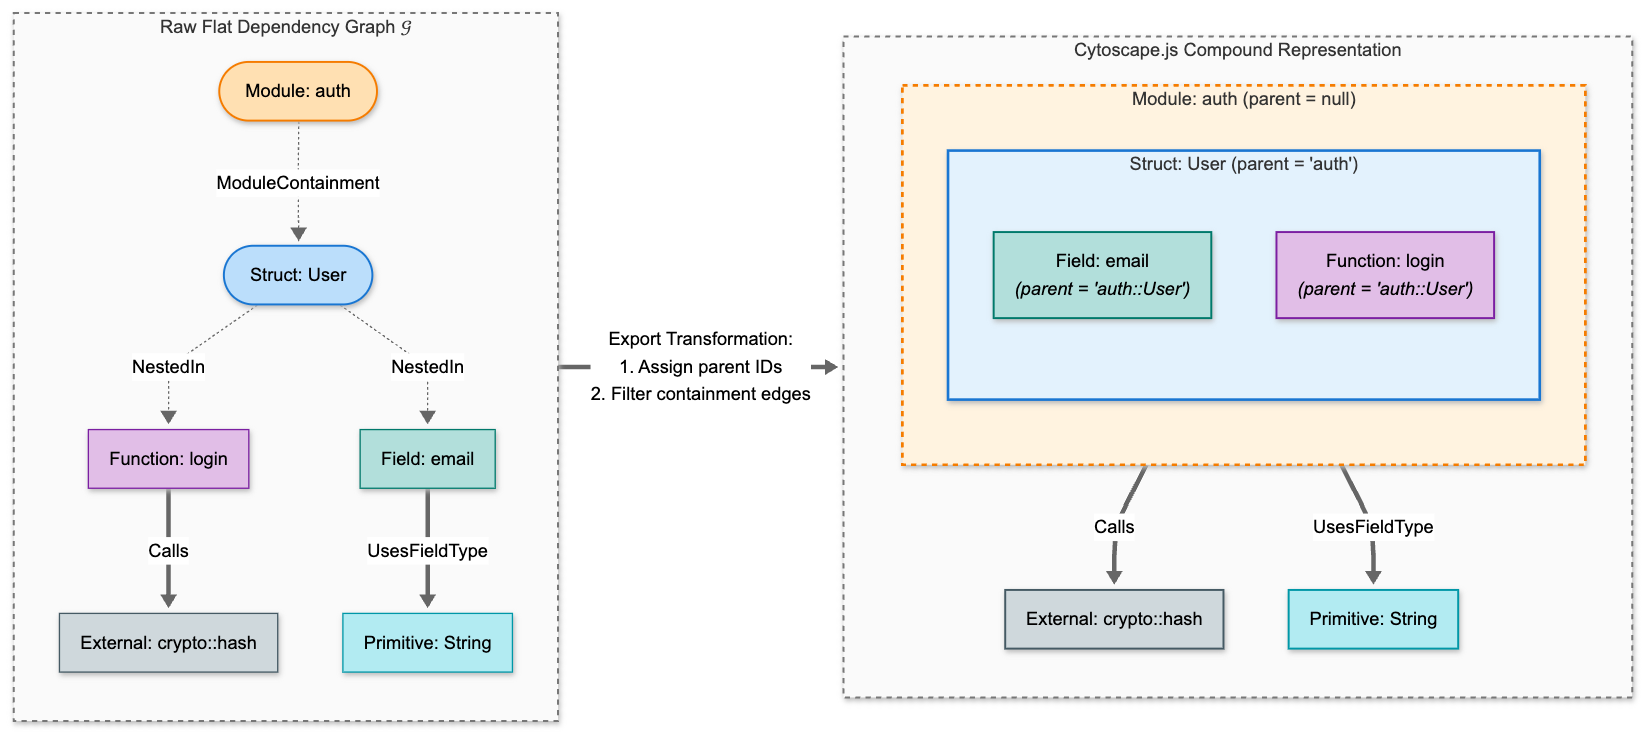
\includegraphics[width=\textwidth]{images/graph_construction/compound_graph_mapping.png}
  \caption{Mapping structural containment to Cytoscape.js compound
    nodes. The raw flat graph (left) connects containers and members
    with explicit \texttt{ModuleContainment} and \texttt{NestedIn}
    edges. The exported representation (right) transforms containment
    into nested bounding boxes via the \texttt{parent} property,
  pruning structural edges and highlighting architectural dependencies.}
  \label{fig:compound_graph_mapping}
\end{figure}

Each exported node carries the following data fields:
\begin{itemize}
  \item \texttt{id}: The fully qualified name, joined with
    \texttt{::} separators (e.g., \texttt{auth::User}).
  \item \texttt{label}: The last segment of the qualified name (e.g.,
    \texttt{User}).
  \item \texttt{type}: The component category (\texttt{Module},
    \texttt{Class}, \texttt{Struct}, \texttt{Function}, etc.).
  \item \texttt{parent}: The \texttt{id} of the enclosing compound
    node, if applicable.
\end{itemize}

Each exported edge carries:
\begin{itemize}
  \item \texttt{source} and \texttt{target}: The \texttt{id}s of the
    source and target nodes.
  \item \texttt{label}: The edge kind as a string (e.g.,
    \texttt{Calls}, \texttt{IsA}).
\end{itemize}

Edges are deduplicated during export using a hash set that tracks the
combination of source, target, and label to prevent visual duplication.

\subsection{The Web-Based Graph Visualizer}

To provide an interactive exploration environment for the generated
graphs, a companion web application was developed using
\textbf{SvelteKit} (Svelte 5) \cite{harris_svelte_2024} and the Cytoscape.js
library. The application communicates with the Rust analyzer through
local API endpoints that invoke the CLI binary and return the
Cytoscape-formatted JSON. The high-level architecture of the
visualization system is depicted in Figure~\ref{fig:visualizer_architecture}.

\begin{figure}[htpb]
  \centering
  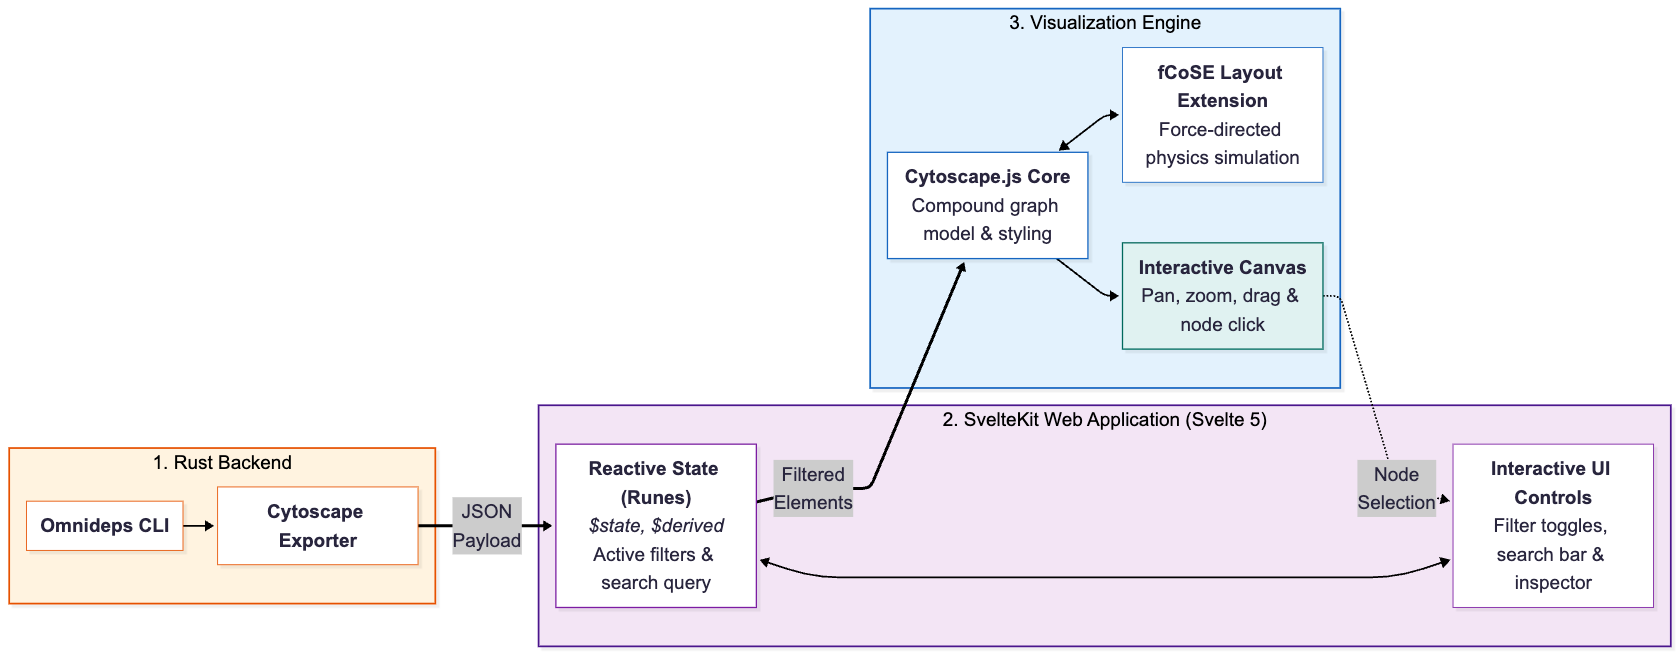
\includegraphics[width=\textwidth]{images/graph_construction/visualizer_architecture.png}
  \caption{Architecture of the interactive graph visualizer. The Rust
    analyzer backend exposes CLI and local HTTP API endpoints
    delivering Cytoscape-formatted JSON payloads. The SvelteKit
    frontend coordinates reactive state management (using Svelte 5
    runes for filter toggles and search queries) with the Cytoscape.js
  canvas and the \texttt{fCoSE} physics layout extension.}
  \label{fig:visualizer_architecture}
\end{figure}

\subsubsection{Graph Layout}

The visualizer employs the \textbf{fCoSE} (Fast Compound Spring
Embedder) layout algorithm \cite{balci_fcose_2022}, a force-directed layout
specifically designed for compound graphs with nested node
hierarchies. The algorithm treats compound nodes as elastic
containers and arranges child nodes within their parent boundaries
while simultaneously optimizing the overall graph topology through
spring-electric forces. Key parameters configured in the application include:
\begin{itemize}
  \item \texttt{quality: ``proof''}: Requests the highest quality
    layout computation.
  \item \texttt{idealEdgeLength}: Controls the target distance
    between connected nodes.
  \item \texttt{nodeRepulsion}: Controls the repulsive force between
    non-adjacent nodes.
  \item \texttt{gravityCompound}: Controls how strongly child nodes
    are pulled toward the center of their parent compound node.
  \item \texttt{packComponents}: Enables compact packing of
    disconnected graph components.
\end{itemize}

\subsubsection{Node and Edge Visual Encoding}

Each node type is rendered with a distinct color, border style, and
geometric shape to enable immediate visual identification:
\begin{itemize}
  \item \textbf{Modules}: Orange (\texttt{\#d35400}), dashed border,
    rendered as compound bounding boxes.
  \item \textbf{Classes and Structs}: Blue (\texttt{\#2980b9}), solid
    border, rendered as compound containers when containing methods or fields.
  \item \textbf{Interfaces and Traits}: Green (\texttt{\#27ae60},
    border \texttt{\#2ecc71}), distinguishing abstract contracts from
    concrete types.
  \item \textbf{Enums and Variants}: Magenta/pink
    (\texttt{\#e84393}), rendered as compound containers for their
    variants (\texttt{EnumVariant}).
  \item \textbf{Functions and Constructors}: Purple
    (\texttt{\#8e44ad}), rendered as ellipses. Functions marked with
    $\mathbb{B}_{ctor} = \text{true}$ receive the specialized type
    tag \texttt{Constructor}.
  \item \textbf{Fields}: Teal (\texttt{\#16a085}), rendered as
    rounded rectangles.
  \item \textbf{Static Variables}: Yellow (\texttt{\#f1c40f}) with
    dark text, differentiating module-level free variables from
    structured fields.
  \item \textbf{Type Aliases}: Violet (\texttt{\#9b59b6}), rendered as diamonds.
  \item \textbf{Primitive Types}: Turquoise (\texttt{\#1abc9c}),
    rendered as hexagons (hidden by default to avoid visual clutter).
  \item \textbf{External Types}: Slate grey (\texttt{\#34495e}),
    rendered with reduced opacity (0.7) and thin border.
\end{itemize}

Edge styling similarly encodes the dependency category through color,
thickness, and line dashing:
\begin{itemize}
  \item \textbf{Inheritance} (\texttt{IsA}): Solid red line (3px,
    \texttt{\#e74c3c}).
  \item \textbf{Implementation} (\texttt{Implements}): Dashed orange
    line (3px, \texttt{\#f39c12}).
  \item \textbf{Calls} (\texttt{Calls}): Solid green line (2px,
    \texttt{\#2ecc71}).
  \item \textbf{Instantiation} (\texttt{Instantiates}): Dashed blue
    line (2px, \texttt{\#3498db}).
  \item \textbf{Field Access} (\texttt{AccessesField}): Dashed amber
    line (2px, \texttt{\#e67e22}).
  \item \textbf{Imports} (\texttt{Imports}): Solid purple line (2px,
    \texttt{\#8e44ad}, opacity 0.8).
  \item \textbf{Auxiliary Annotations and Aliasing}
    (\texttt{AnnotatedWith}, \texttt{Aliases}): Dotted magenta line
    (2px, \texttt{\#ff00ff}).
  \item \textbf{Type Casts} (\texttt{CastsTo}): Dashed cyan line
    (2px, \texttt{\#00a8ff}).
  \item \textbf{Type Usage} (\texttt{UsesFieldType},
      \texttt{UsesLocalType}, \texttt{UsesParamType},
    \texttt{UsesReturnType}): Dotted grey line (\texttt{\#95a5a6}, opacity 0.7).
  \item \textbf{Containment} (\texttt{ModuleContainment},
    \texttt{NestedIn}): Thin grey line (1px, \texttt{\#7f8c8d},
    opacity 0.5), shown only when compound container grouping is toggled off.
\end{itemize}

\subsubsection{Interactive Features}

To facilitate software architecture exploration and mitigate the
visual clutter typical of large dependency networks, the visualizer
implements interactive exploration and filtering techniques
\cite{diehl_software_2007}:

\begin{itemize}
  \item \textbf{Node Search}: A text input field filters the graph in
    real time. Nodes whose labels match the query (case-insensitive
    substring match) are highlighted, while all other nodes are
    visually dimmed. Matching nodes and their ancestor compound
    containers remain visible to preserve spatial context.
  \item \textbf{Node Inspection}: Tapping a node opens a detail
    sidebar displaying the node's type, full qualified name, and a
    breakdown of its incoming and outgoing edges, grouped by edge
    kind. Each related node in the sidebar is clickable, allowing
    navigation through the graph.
  \item \textbf{Neighborhood Focus}: When a node is tapped, the graph
    automatically dims all nodes and edges except the selected node,
    its direct neighborhood (connected nodes and their mutual edges),
    and its ancestor/descendant compound containers.
  \item \textbf{Edge Filtering}: The control panel provides two
    groups of toggle switches for edge filtering:
    \begin{itemize}
      \item \textit{Structural filters}: \texttt{IsA},
        \texttt{Implements}, \texttt{Imports},
        \texttt{UsesFieldType}, \texttt{UsesParamType},
        \texttt{UsesReturnType}, \texttt{UsesLocalType},
        \texttt{NestedIn}, \texttt{ModuleContainment}, \texttt{AnnotatedWith}.
      \item \textit{Behavioral filters}: \texttt{Calls},
        \texttt{Instantiates}, \texttt{AccessesField}.
    \end{itemize}
    Each filter can be toggled independently, with a master toggle
    for each group. The filtering logic operates in batch mode: edges
    of disabled kinds are hidden, and edges whose source or target
    node is itself hidden are also suppressed.
  \item \textbf{Node Type Filtering}: Separate toggles allow hiding
    or showing entire categories of nodes (e.g., all \texttt{Module}
      nodes, all \texttt{External} nodes, all \texttt{Primitive}
    nodes). By default, \texttt{Primitive} nodes are hidden to reduce noise.
  \item \textbf{JSON Export}: Two export options are provided:
    exporting the Cytoscape-formatted elements (for re-importing into
    visualization tools) and exporting the raw analyzer JSON output
    (for programmatic consumption).
\end{itemize}
